This panel is provided for the user to specify multiple existing SimCenter
event files.  If more than one event is specified it is done to
provide the UQ engine with a discrete set of events to choose
from\textemdash it is not done with the intention of specifying that
one event follows another.  The panel presented to the user
is shown in \Cref{fig:SC_event_panel}.

\begin{figure}[!htbp]
  \centering {
    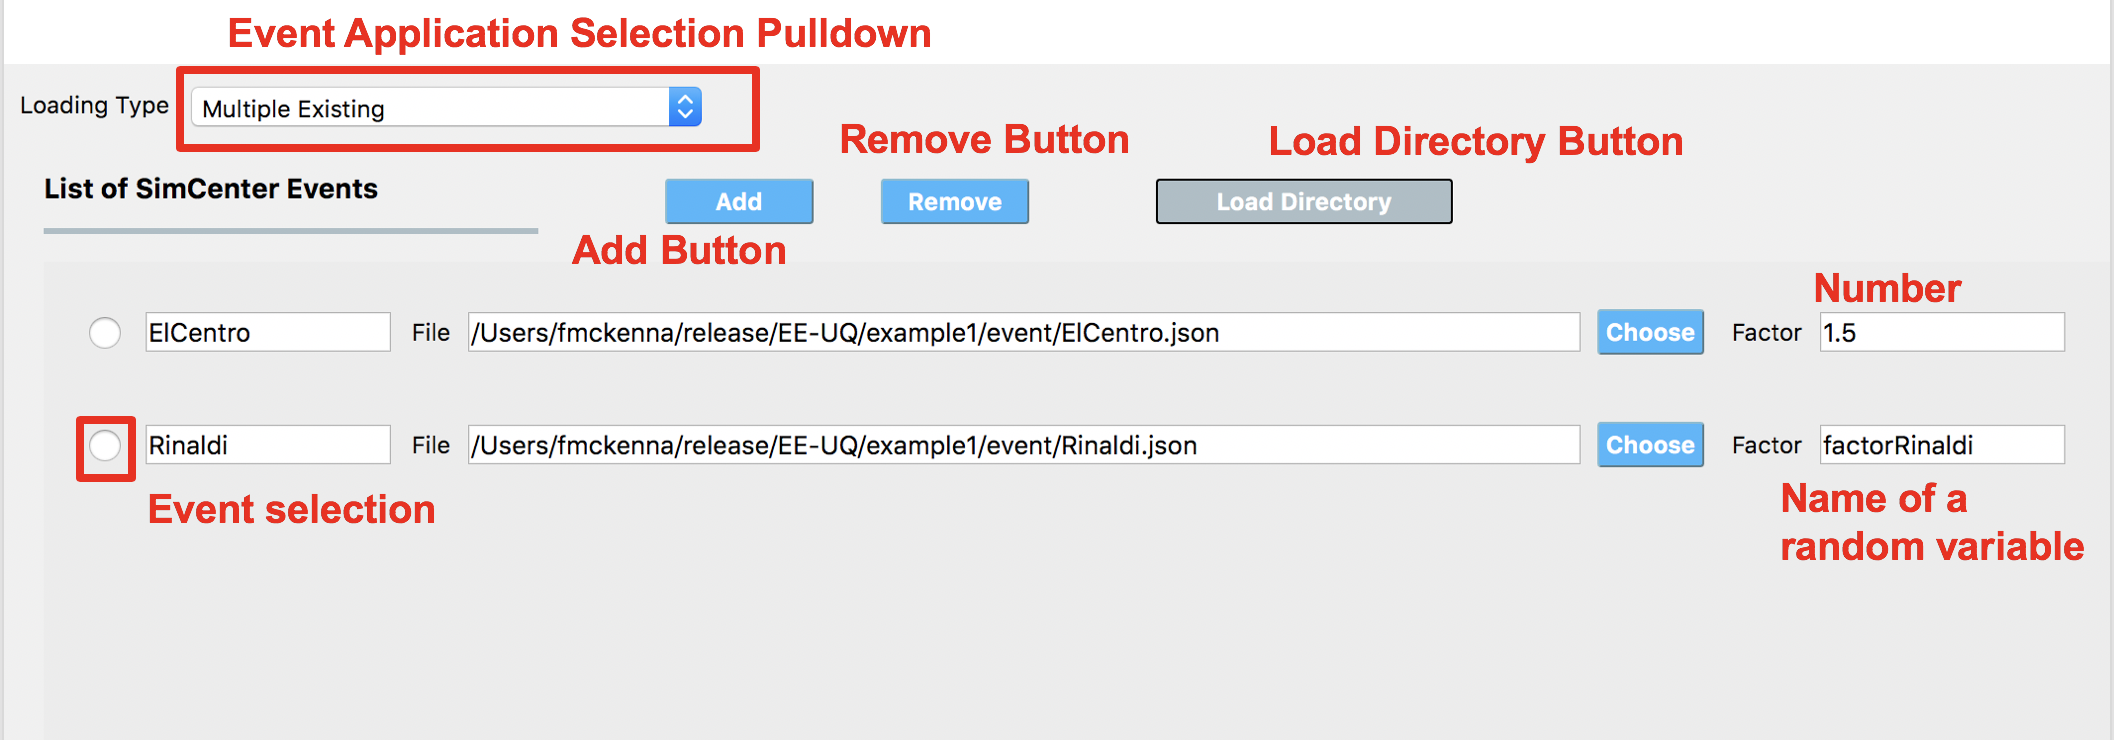
\includegraphics[width=0.8\textwidth]
    {usage/figures/multipleExisting.png} }
  \caption{Multiple Existing (SimCenter) Events }
  \label{fig:SC_event_panel}
\end{figure}

Use the \texttt{Add} button to add a new event. This adds an empty
event to the panel. Pressing the button multiple times will keep
adding events to the panel. \Cref{fig:SC_event_panel} shows the state after
the button has been pressed twice, and data entered to load the El Centro
and Rinaldi Events.

The path to the event file can be entered manually, or using the \texttt{Choose} button for convenience. Pushing the button brings up a typical file search screen. By default, a scale factor of 1.0 is assigned to the event.  The user
can change this to another floating point value (DO NOT USE INTEGER), and they can define the scale factor as a random variable by
entering a variable name, such as \texttt{factorRinaldi} for the second event in \Cref{fig:SC_event_panel}.

Note: the name of the random variable must not start with a number, or contain any spaces or special characters, such as -, +, \%, etc.

The \texttt{Remove} button is used to remove events. To remove an
event, the user must first select events they wish to remove,
which is done by clicking in the small circle at the left side of the event frame. All of the selected events are removed when the \texttt{Remove} button is pressed.

The \texttt{Load Directory} button provides a convenient method to load multiple events. All event files shall first
be placed into the same folder. We recommend to put the files in a folder of their own, with no other files besides the earthquake events in it. After pressing the \texttt{Load Directory} button, the user will be able to choose the directory that contains the files, and the
application will load all event files (i.e., every file with a \texttt{.json} 
extension) into the widget automatically. 

Initially, every
event will be given a load factor of 1.0. Load factors can be assigned automatically by preparing a \texttt{Records.txt} file in the directory with the events. Each line in the \texttt{Records.txt} shall represent one event file, and contain two comma separated values: the event file name and the desired scale factor. The application will open that file automatically and assign the prescribed load factors to the events. Using a \texttt{Records.txt} file also allows users to load only a subset of the events from a folder by listing only those in the file. An example \texttt{Records.txt} is shown below:

\begin{verbatim}
ElCentro.json,1.5
Rinaldi.json,2.0
\end{verbatim}

Random Variables: Scale factors can be defined as being random variables by entering a string in the factor field. The variable name entered will appear as a Random Variable in the UQ panel and the user must specify its distribution there. If multiple
events are specified, the event itself will be also be treated as a random
variable, with each event being part of the discrete set of possible
events. For this discrete set the user does not define a distribution as this is done automatically.
